\documentclass[10pt,landscape,a4paper]{article}
\usepackage[utf8]{inputenc}
\usepackage[ngerman]{babel}
\usepackage[T1]{fontenc}
%\usepackage[LY1,T1]{fontenc}
%\usepackage{frutigernext}
%\usepackage[lf,minionint]{MinionPro}
\usepackage{tikz}
\usetikzlibrary{shapes,positioning,arrows,fit,calc,graphs,graphs.standard}
\usepackage[nosf]{kpfonts}
\usepackage[t1]{sourcesanspro}
\usepackage{multicol}
\usepackage{wrapfig}
\usepackage[top=0mm,bottom=1mm,left=0mm,right=1mm]{geometry}
\usepackage[framemethod=tikz]{mdframed}
\usepackage{microtype}
\usepackage{pdfpages}

\let\bar\overline

\definecolor{myblue}{cmyk}{1,.72,0,.38}

\def\firstcircle{(0,0) circle (1.5cm)}
\def\secondcircle{(0:2cm) circle (1.5cm)}

\colorlet{circle edge}{myblue}
\colorlet{circle area}{myblue!5}

\tikzset{filled/.style={fill=circle area, draw=circle edge, thick},
    outline/.style={draw=circle edge, thick}}
    
\pgfdeclarelayer{background}
\pgfsetlayers{background,main}

\everymath\expandafter{\the\everymath \color{myblue}}
\everydisplay\expandafter{\the\everydisplay \color{myblue}}

\renewcommand{\baselinestretch}{.8}
\pagestyle{empty}

\global\mdfdefinestyle{header}{%
linecolor=gray,linewidth=1pt,%
leftmargin=0mm,rightmargin=0mm,skipbelow=0mm,skipabove=0mm,
}

\newcommand{\header}{
\begin{mdframed}[style=header]
\footnotesize
\sffamily
CS2106 (Operating System) Cheatsheet\\
Zhang Yuntong, Page \thepage~out of~2
\end{mdframed}
}

\makeatletter % Author: https://tex.stackexchange.com/questions/218587/how-to-set-one-header-for-each-page-using-multicols
\renewcommand{\section}{\@startsection{section}{1}{0mm}%
                                {.2ex}%
                                {.2ex}%x
                                {\color{myblue}\sffamily\small\bfseries}}
\renewcommand{\subsection}{\@startsection{subsection}{1}{0mm}%
                                {.2ex}%
                                {.2ex}%x
                                {\sffamily\bfseries}}



\def\multi@column@out{%
   \ifnum\outputpenalty <-\@M
   \speci@ls \else
   \ifvoid\colbreak@box\else
     \mult@info\@ne{Re-adding forced
               break(s) for splitting}%
     \setbox\@cclv\vbox{%
        \unvbox\colbreak@box
        \penalty-\@Mv\unvbox\@cclv}%
   \fi
   \splittopskip\topskip
   \splitmaxdepth\maxdepth
   \dimen@\@colroom
   \divide\skip\footins\col@number
   \ifvoid\footins \else
      \leave@mult@footins
   \fi
   \let\ifshr@kingsaved\ifshr@king
   \ifvbox \@kludgeins
     \advance \dimen@ -\ht\@kludgeins
     \ifdim \wd\@kludgeins>\z@
        \shr@nkingtrue
     \fi
   \fi
   \process@cols\mult@gfirstbox{%
%%%%% START CHANGE
\ifnum\count@=\numexpr\mult@rightbox+2\relax
          \setbox\count@\vsplit\@cclv to \dimexpr \dimen@-1cm\relax
\setbox\count@\vbox to \dimen@{\vbox to 1cm{\header}\unvbox\count@\vss}%
\else
      \setbox\count@\vsplit\@cclv to \dimen@
\fi
%%%%% END CHANGE
            \set@keptmarks
            \setbox\count@
                 \vbox to\dimen@
                  {\unvbox\count@
                   \remove@discardable@items
                   \ifshr@nking\vfill\fi}%
           }%
   \setbox\mult@rightbox
       \vsplit\@cclv to\dimen@
   \set@keptmarks
   \setbox\mult@rightbox\vbox to\dimen@
          {\unvbox\mult@rightbox
           \remove@discardable@items
           \ifshr@nking\vfill\fi}%
   \let\ifshr@king\ifshr@kingsaved
   \ifvoid\@cclv \else
       \unvbox\@cclv
       \ifnum\outputpenalty=\@M
       \else
          \penalty\outputpenalty
       \fi
       \ifvoid\footins\else
         \PackageWarning{multicol}%
          {I moved some lines to
           the next page.\MessageBreak
           Footnotes on page
           \thepage\space might be wrong}%
       \fi
       \ifnum \c@tracingmulticols>\thr@@
                    \hrule\allowbreak \fi
   \fi
   \ifx\@empty\kept@firstmark
      \let\firstmark\kept@topmark
      \let\botmark\kept@topmark
   \else
      \let\firstmark\kept@firstmark
      \let\botmark\kept@botmark
   \fi
   \let\topmark\kept@topmark
   \mult@info\tw@
        {Use kept top mark:\MessageBreak
          \meaning\kept@topmark
         \MessageBreak
         Use kept first mark:\MessageBreak
          \meaning\kept@firstmark
        \MessageBreak
         Use kept bot mark:\MessageBreak
          \meaning\kept@botmark
        \MessageBreak
         Produce first mark:\MessageBreak
          \meaning\firstmark
        \MessageBreak
        Produce bot mark:\MessageBreak
          \meaning\botmark
         \@gobbletwo}%
   \setbox\@cclv\vbox{\unvbox\partial@page
                      \page@sofar}%
   \@makecol\@outputpage
     \global\let\kept@topmark\botmark
     \global\let\kept@firstmark\@empty
     \global\let\kept@botmark\@empty
     \mult@info\tw@
        {(Re)Init top mark:\MessageBreak
         \meaning\kept@topmark
         \@gobbletwo}%
   \global\@colroom\@colht
   \global \@mparbottom \z@
   \process@deferreds
   \@whilesw\if@fcolmade\fi{\@outputpage
      \global\@colroom\@colht
      \process@deferreds}%
   \mult@info\@ne
     {Colroom:\MessageBreak
      \the\@colht\space
              after float space removed
              = \the\@colroom \@gobble}%
    \set@mult@vsize \global
  \fi}

\makeatother
\setlength{\parindent}{0pt}

\begin{document}
%\footnotesize
\small
\begin{multicols*}{5}
\section{Introduction to OS}
\emph{Monolithic:} One big special program. Unix variants and Windows NT/XP. (+) Well understood,good performance. (-) highly coupled components.\\
\emph{Microkernel:} Small and clean. Only provides basic and essential facilities (IPC, scheduling, interrupt handler). Higher level services built on top and run as server process outside of the OS (use IPC to communicate). (+) Kernel extensible and better isolation \& protection between kernel and higher level services. (-) lower performance.
\section{System Calls}
\subsection*{General System Call Mechanism}
Library call places the syscall \# in designated register, executes TRAP/SYSCALL to switch from user mode to kernel mode. Dispatcher determines syscall handler using syscall \# as index. Syscall handler executed, return control to library call and switch to user mode when finished.

\subsection*{Exception and Interrupts}
\emph{Exception:} Synchronous (error in program execution).\emph{Interrupt:} Asynchronous. Some portion of state saving done by hardware. Save state/registers in special interrupt stack.  Usually special return from interrupt instruction. Non-maskable interrupt - always handled; Maskable interrupt - can be enabled or disabled (x86: CLI, STI). Vectored interrupt - array of interrupt handlers called by indexing interrupt \# (x86: int n). General interrupt handler - some way to determine type (using 'cause' register)\\
int system(const char *command\_line): creates a shell to run command line.
\section{Process Abstraction}
\emph{PCB/PTE:} The entire execution context (hardware, memory, OS) for a process. \emph{Process Table:} Kernel maintains PCB for all processes in the process table.
\section{Process Abstraction in Unix}
\emph{void exit(int status):} released on exit: memory, file descriptors. not yet releasable: PID, status, process accounting info, PTE. Child processes are inherited by init process. Parent sent SIGCHLD signal, status returned to parent using wait(). Cleanup: flush and close open streams from C stdio. Calls (several) exit handlers specified by program. Calls \_exit(status) after standard C cleanup.

\subsection*{Parent-Child Synchronization}
\emph{int wait(int *status):} Returns PID of terminated child. Parent blocks until at least one child terminates. Cleans up remainder of child system resources. Kill zombie process. \emph{waitid():} Wait for any child process to change status.\\
\emph{init process:} Created in kernel at boot up time (PID=1). \emph{Zombie process:} Parent terminates before child, init becomes 'pseudo' parent, init utilizes wait() to cleanup, or; Child terminates before parent but parent didn't call wait(), child process becomes zombie, can fill up process table, may need reboot.

\subsection*{Implementation Issues on fork()}
Copy on Write: duplicate a page when it is written to; otherwise parent and child share the same page. CoW with paged VM: Share single page by having PTEs with same frame. Share read-only pages. Duplicate and make new page copy on write, PTE changed to new page and make page writable.
\section{Process Scheduling}
OS incurs overhead in context switch. Batch processing, Interactive, Real time processing.

\subsection*{Scheduling for Batch Processing}
\emph{Criteria:} turnaround time (finish-arrival time), throughput (number of tasks finished per unit time), CPU utilization\\
\emph{First-Come First-Served (FCFS):} Blocked task removed from FIFO queue, only placed at back of queue when it's ready again. (+) No stavation.(-) Convoy effect (First task is CPU-Bound and followed by a number of IO-Bound tasks).\\
\emph{Shortest Job First (SJF):} $Predicted_{n+1}=\alpha Actual_n + (1-\alpha)Predicted_n$ (+) Smallest average waiting time. (-) Starvation possible (for long job).\\
\emph{Shortest Remaining Time (SRT):} New job with shorter remaining time can preempt current job. (Good service for short job even when arriving late)

\subsection*{Scheduling for Interactive Systems}
Preemptive, scheduler runs periodically (from timer interrupt).\\
\emph{Criteria:} response time, predictability (less variation in resp time).\\
\emph{Round Robin (RR):} Preemptive version of FCFS (ready tasks placed at back of queue, blocked tasks moved to other queue). (+) Reponse time guarantee - n tasks quantum q, time before a task gets CPU bounded by $(n-1)q$. Big quantum: better CPU utilization, longer waiting time. Small quantum: Bigger overhead, shorter waiting time.\\
\emph{Priority Scheduling:} Preemptive version: high priority proc can preempt running proc. Non-preemptive version: late coming high priority proc has to wait for next round of schduling. (-) Low priority proc can starve (worse in preemptive) -> decrease prioirty of current proc after each time quantum. (-) Hard to control CPU time. (-) Priority inversion: Lower priority task preempts higher priority task (high priority task requires resources locked by even lower priority task).\\
\emph{Multi-level Feedback Queue (MLFQ):} Adaptive, reduce reponse time for IO-bound process, turnaround time for CPU bound process.\\
Basic rules:\\
Priority(A) > Priority(B) -> A runs\\
Priority(A) == Priority(B) -> A, B in RR\\
Priority setting/changing rules:\\
New job -> Highest priority\\
Use up timeslice -> Priority reduced\\
Give up/blocks -> Priority retained\\
\emph{Lottery Scheduling:} Give out 'lottery tickets' to processes for various system resources. Choose ticket randomly and grant winner the resource. (+) Responsive. (+) Good lvl of control (parent gives tickets to child). (+) Simple implementation.
\section{Process Scheduling in Unix}
\subsection*{Traditional Unix Process Priority}
\emph{nice:} -20 to 19, default 0. priority=base+f(nice)+g(cpu usage estimate), g() is decay factor to reduce importance of long process.

\subsection*{Multi-level Feedback Queues}
Dynamic adjustments with scheduling heuristics: age of proc, I/O boost (for interactive process), boost priority of foreground window (WinNT), system load effects.

\subsection*{Linux Scheduling}
\emph{Multi-level feedback queue:} level 0: Normal Time Sharing (SCHED\_OTHER). level 1 to 99: Real-time FIFO(SCHED\_FIFO) and Real-time Round Robin (SCHED\_RR).\\
\emph{SCHED\_FIFO:} scheduling occurs only when higher priority RT arrives or voluntary yield. (timer interrupt used only for high priority to preempt).\\
\emph{SCHED \_RR:} preemptive. Preemption by higher priority RT tasks also.\\
\emph{SCHED\_OTHER:} nice priorities + dynamic feedback adjustments. Only run if no RT task ready.\\
Static priorities (RT priorities) not changed by scheduler, dynamic priority used for SCHED\_OTHER tasks and changed by system. -> Static RT priority > Dynamic priority

\subsection*{Tickless}
In new Linux kernels+WinNT. Only use timer interrupt when needed (not in sleep mode, adjust tick to next closest timer event). Tickless isn't no ticks but dynamic ticks.
\section{Memory Abstraction}
\emph{int brk(void *end\_data\_segment):} how to deallocate?\\
\emph{void *sbrk(ptrdiff\_t brk\_increment):} argument is signed integer, return previous break value.\\
\emph{void *malloc(size\_t size):} returns pointer to new memory region of size bytes.\\
\emph{void free(void *ptr):} ptr must have been originally from malloc/calloc.\\
\emph{void *calloc(size\_t nitems, size\_t size):} sets allocated memory to zero (malloc doesn't).
\section{Contiguous Memory Allocation}
\subsection*{Contiguous Memory Management}
\emph{Fixed-size partition:} (-) internal fragmentation. (-) external fragmentation (total unused memory > request size but no partition fits)\\
\emph{Dynamic partition:} OS keeps track of occupied and free regions, performs splitting and merging. (+) no internal fragmentation (by splitting). (-) external fragmentation\\
\emph{Relocation \& compaction:} Move partitions around to remove external fragmentation. (-) data which are addresses may refer to wrong address after relocation.

\subsection*{Dynamic Memory Allocation Algorithms}
\emph{Sequential Fit:} In free block: doubly linked list+size=~3 words for bookkeeping (minimum free block size)\\
First fit: (-) front list split more, many small blocks at start\\
Best fit: find smallest fitting block. (-) need searching whole list. (-) bad external fragmentation with many tiny blocks. (+) experimentally good memory use results.\\
Next fit: search from previously searched position. (+) avoids accumulation of small blocks at start. (-) poor locality affects caches.\\
Freeing a block: boundary tag optimization can coalesce in constant time.\\
\emph{Buddy System:}\\
avail[i] records a free list of blocks of size $2^i$ (NULL means no free blocks). Splitting $xx..xx00..00$ ->$xx..xx00..00$ and $xx..xx10..00$. Find buddies for block of size $2^i$ -> flip bit at position $i+1$ from right to find buddy address. May have smallest allocated block size. (avail[0] for illustration)\\
Buddy allocation n: find smallest i for $2^i \geqslant n$. If avail[i] not empty, select free block there; else, find free block $b$ from smallest avail[k] where $k>i$, split $b$ until avail[i] has block.\\
Buddy deallocation p: find buddy p'. If p' not free, add p to avail list; else, coalesce p and p' and free it recursively.
\section{Logical Addressing Schemes}
VM cost: Badly behaved program causes thrashing.

\subsection*{Segmentation for Address Translation}
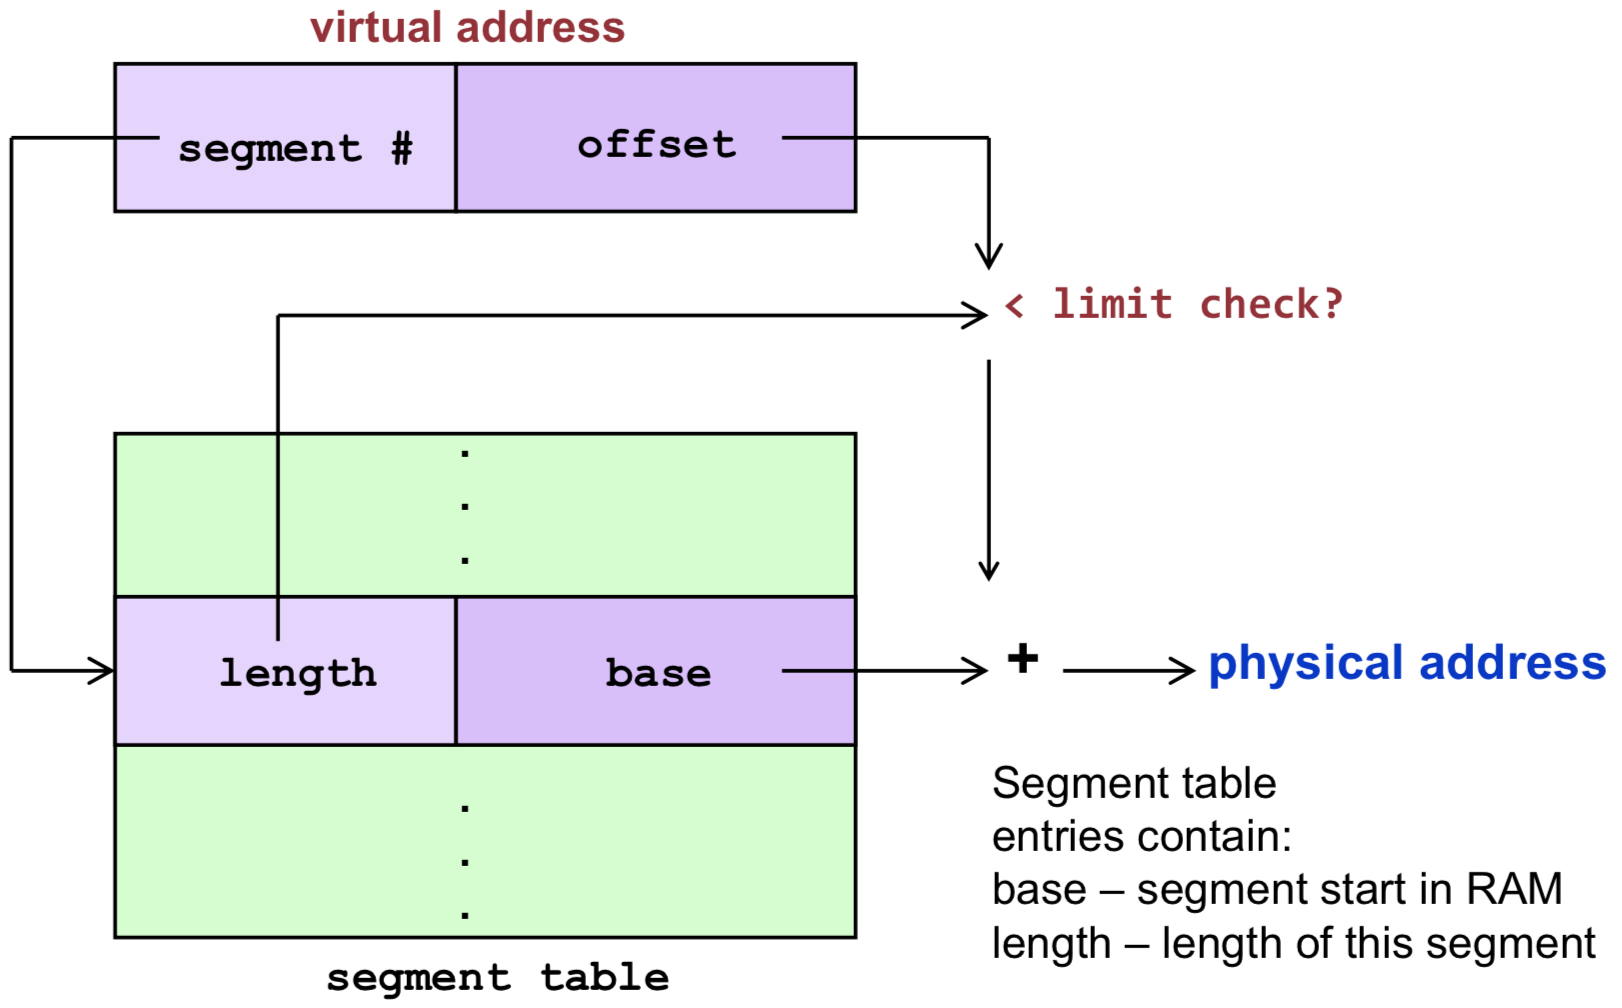
\includegraphics[width=0.75\linewidth]{images/segmentation-scheme}\\
permission info (read, write, exec -> invalid operation leads to seg fault).\\
(-)external fragmentation (but easier compaction), resizing causes framentation problems, may require explicitly selecting segments, swapping overhead high for large segments.

\subsection*{Paging for Address Translation}
Internal fragmentation, no external fragmentation. Rather than resizing, just use more pages. Overhead of page transfer to/from swap is on the order of few disk blocks.\\
\emph{Memory Sharing:} VM not needed for sharing, but allows logical address to be different and still share.\\
\emph{Direct Paging:}\\
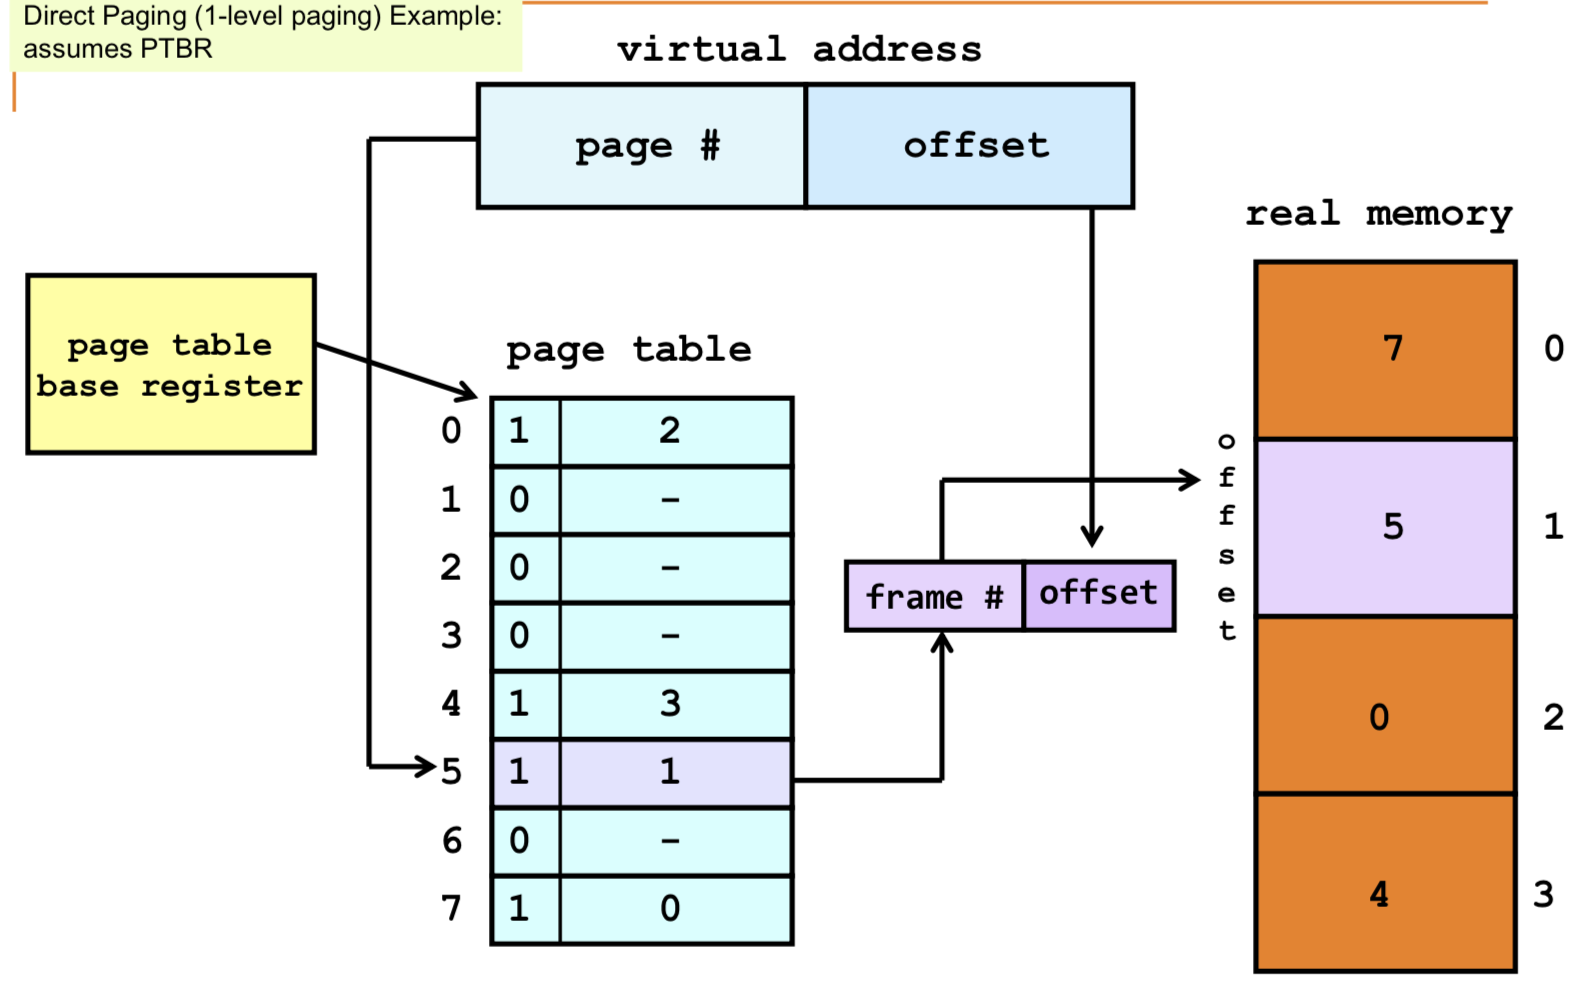
\includegraphics[width=0.8\linewidth]{images/direct-paging}\\
Overhead: page table size too big (same regardless of process memory usage)\\
\emph{2-level Paging:} save space\\
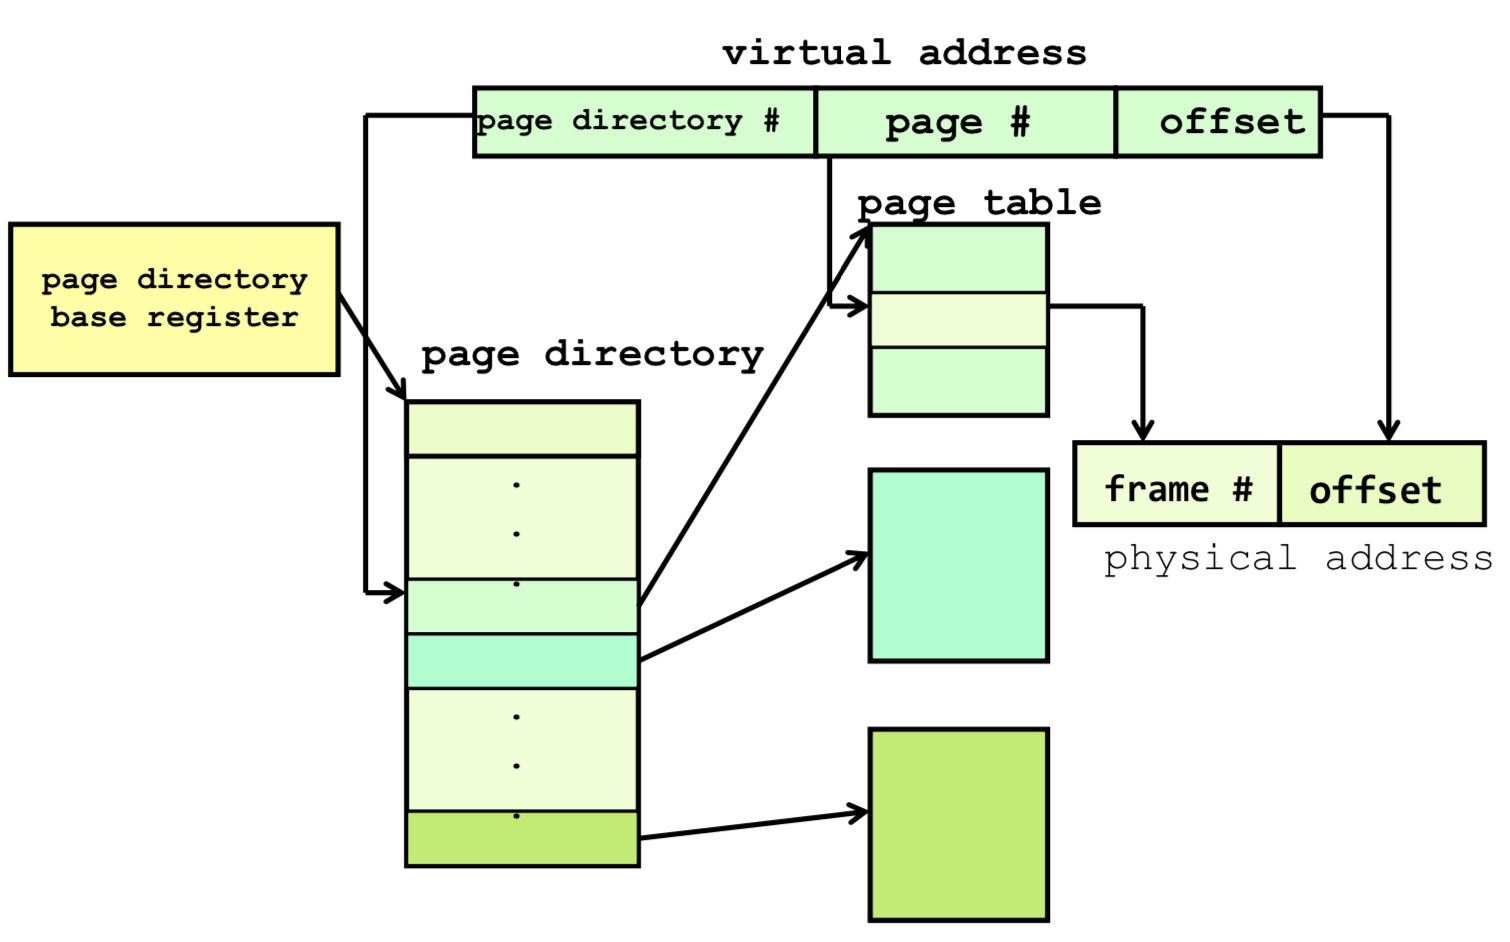
\includegraphics[width=0.8\linewidth]{images/2-level-paging}\\
\emph{Multi-level Paging:} tree with k levels for k-level paging, space savings when tree not complete. Pages tables can be in VM and be paged.\\
\emph{x86 hybrid paging: segmentation+paging:}\\
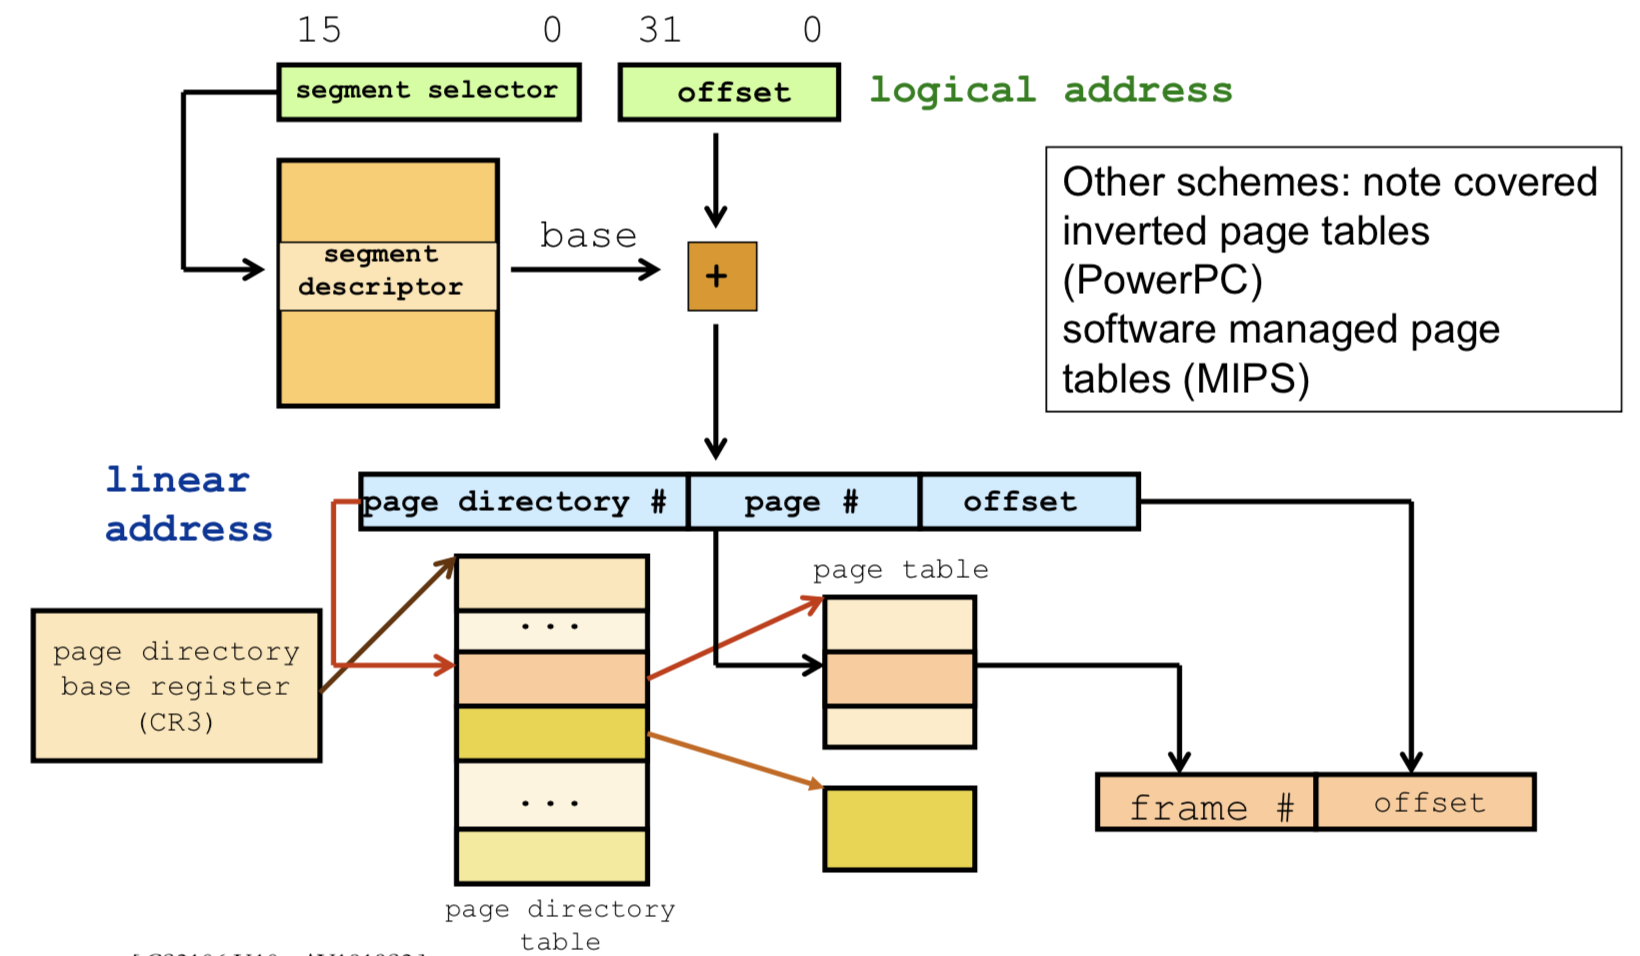
\includegraphics[width=0.8\linewidth]{images/x86-paging}

\subsection*{Page Table Entries (multi-level paging)}
\emph{Non-leaf nodes:} address of next level page table, valid bit. \emph{Leaf nodes:} frame, valid(present) bit - page present in RAM, dirty(modified) bit - set when page is written, referenced bit - set when page is used, protection bits - read/write/exec.

\subsection*{Translation Lookaside Buffer (TLB)}
$memory\_access\_time=m+(1-p) \ast 1+pkm) \approx m$ (k-level paging). Without cache: $(k+1)m$ (p=1). Context switch -> TLB flush, just invalidate entire TLB cache. x86: write to register CR3(PDBR) flushes TLB.
\section{Virtual Memory Management}
\subsection*{Page Fault}
HW virtual address translation: transparent if succeeds (frame in RAM, no protection violation) (common case), page fault exception if fails.\\
Page fault cases: page not present (valid bit off, OS handles, recursion if dealing with fault in page tables), protection error (OS generates software exception - SIGSEGV (seg fault) or SIGBUS), page not used (valid bit off, could be an auto expanding segment like stack).\\
Reset page table may need update multi-level tables.

\subsection*{Page Placement Policy: any frame}
\subsection*{Page Fetch Policy}
\emph{Demand paging:} only faulting page is fetched. \emph{Prepaging:} other pages can be fetched on page fault. Can also be loaded when starting process.

\subsection*{Page Replacement Algorithms}
Incoming page can be from swap or executable file. If page to be replaced is dirty, need to write back to swap; if clean, can be discarded. Good algorithm have very few page faults: $T_{access}=(1-p)T_{mem}+pT_{page\_fault}$.\\
\emph{Optimal Page Replacement (OPT):} Replace page that will not be used again for the longest time, guarantees min page faults.\
\emph{FIFO:} Evict oldest memory page. (+) simple implementation (OS maintains queue of resident page no.) (-) Belady's Anomaly (more frames, more page faults, since doesn't exploit temporal locality).\\
\emph{Least Recently used (LRU):} Replace page that has not been used in longest time (temporal locality). (-) Hard to implement. Appr. 1: counter, PTE with time-of-use field(forever increasing may overflow), need to search through all pages. Appr. 2: stack of page no. If X referenced, remove from stack and push on top. Replace page at stack bottom.\\
\emph{Second-Chance (CLOCK):}\\
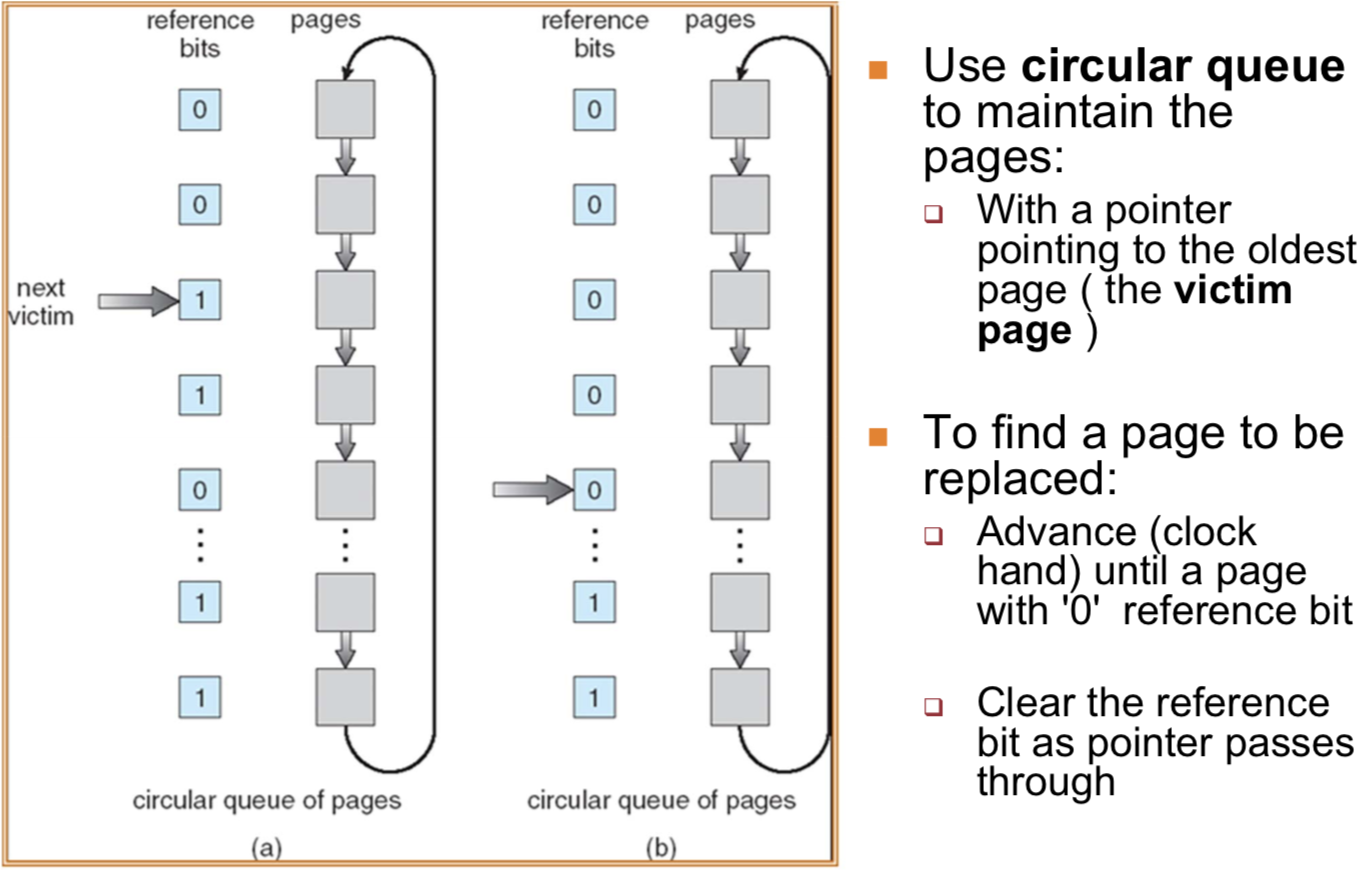
\includegraphics[width=0.8\linewidth]{images/second-chance-page-replacement}\\
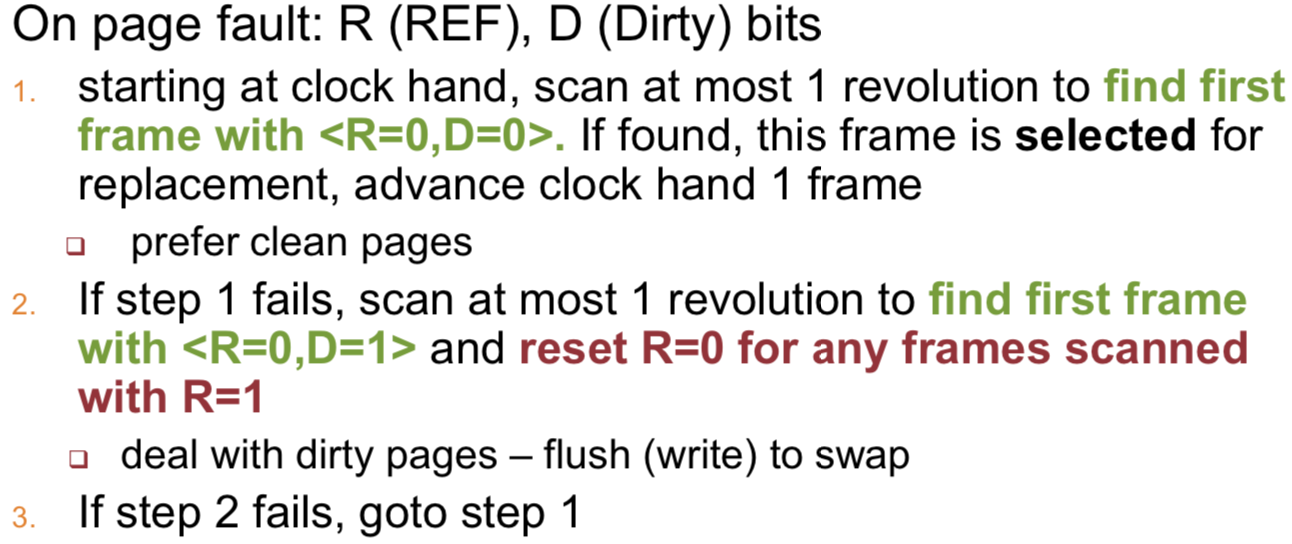
\includegraphics[width=0.9\linewidth]{images/clock_algo}

\subsection*{Frame Allocation}
Equal allocation(N/M), Proportional allocation($size_p/size_{total}*N)$.\\
Local replacement: (+) Stable performance between multiple runs, (-) not enough frame hinder progress. Global replacement: (+) self-adjustment between processes, (-) bad process affects others.\emph{Thrashing:} not enough frame, global -> cascading thrashing, local -> single process hogs I/O.\\
\emph{Working Set Model:}\\
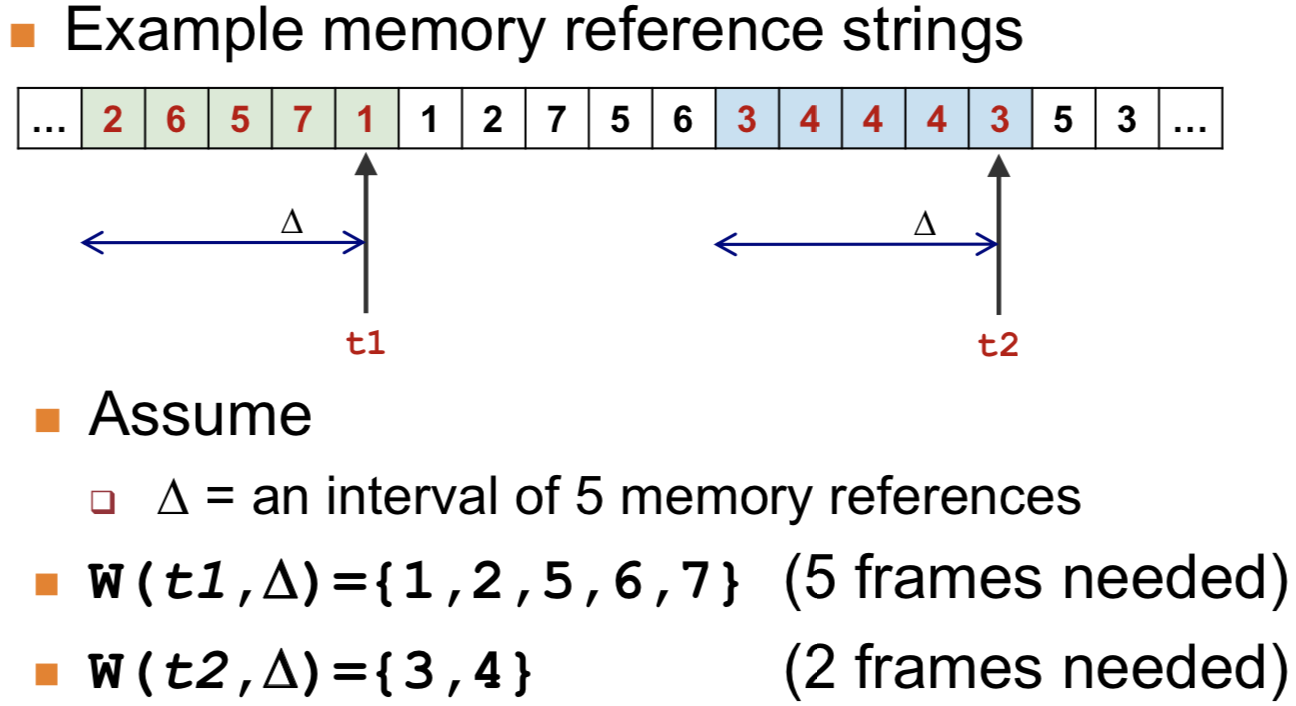
\includegraphics[width=0.75\linewidth]{images/working-set-example}\\
$\Delta$: too small -> miss page in current locality, too big : contains page from different locality.
\section{File System Introduction}
\subsection*{File}
\emph{MSDOS file names:} <name>.<extension> : name 9 char, extension 3 char. Letters converted to uppercase. Reserved con, prn, nul...\\

\includegraphics[width=0.75\linewidth]{images/char-set-msdos}\\
\emph{Type:} regular(ASCII, binary), directories, speical files(devices, symbolic links, named pipes). Distinguishing: extension(Win), magic number(Unix).
\emph{Protection:} Access control list, Permission bits(owner, group, other).\\
\emph{Structure:} array of bytes, fixed length record(instant access), variable length record(hard to locate).\\
\emph{Access method:} sequential access(rewound), random access(read, seek), direct access(on fixed length record, general random on record).

\subsection*{Directory}
Single-level, tree-structured (every node has only one parent), DAG (aliases, appear in multiple directories), general graph (achieved with symbolic link, infinite path possible -> maximum traversal limit in Unix).\\
\emph{Unix symbolic link:} Special link file contains path name. ln -s. Recursive. Win: shortcut does not re-expand further(not recursive).
\section{File System Unix}
\emph{unified I/O:} many types of files but same syscalls: data, pipe, devices, proc...\\
int open(char *path, int flags [, mode]): returns -1 if fail, >=0 for file descriptor. mode is new file permissions. Open checks permissions. Default fd: STDIN(0), STDOUT(1), STDERR(2)\\
\emph{fd sharing:} After fork, fd value is copied, internal kernel file object and file offset are shared.\\
int read(int fd, void *buf, int n): return no. of bytes read, <n means reach EOF. sequential read.\\
int write(int fd, void *buf, int n): return -1 if error(exceeds file size limit, quota, disk space), >=0 for no. of bytes written. sequential write.\\
off\_t lseek(int fd, off\_t offset, int whence): Random I/O. Move file offset, return -1 if error, >=0 for absolute offset. Offset can be +ve or -ve, whence can be SEEK\_SET, SEEK\_CUR, SEEK\_END. Can create holes with implicit zeroes.\\
int close(int fd): fd can be reused later. Process termination automatically closes all open files.
\section{File System Implementation}
\subsection*{File Block Allocation}
\emph{Contiguous:} (+) Simple to keep track(start \#+length), fast access. (-) external fragmenation, specify file size in advance.\\
\emph{Linked List:} Store file start end. (+) No fragmentation. (-) slow random access(disk speed pointer), part of block used for pointer.\\
\emph{Linked List V2.0:} Move all block pointers to File Allocation Table(FAT)(in memory). (+) Faster random access(traversal in memory). (-) FAT size depends on disk size, consumes memory.\\
\emph{Indexed allocation:} Linked scheme(linked list of index blocks), multilevel index(1st lvl index block points to several 2nd level index blocks), combined scheme.

\subsection*{Free Space Management}
Linked list(linked indexed representation), array(compress to bitmap).\\
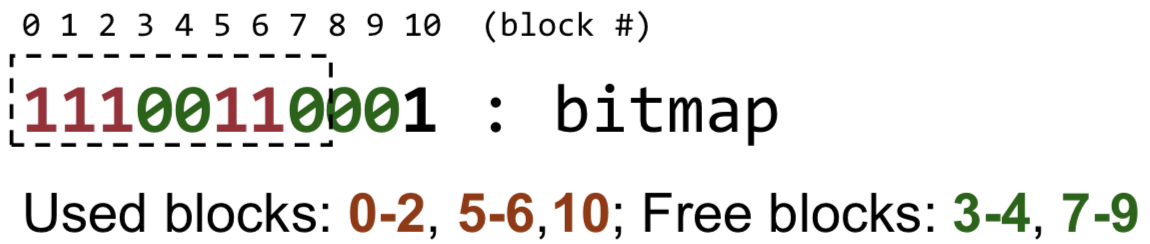
\includegraphics[width=0.75\linewidth]{images/bitmap-free-block}

\subsection*{MSDOS}
FAT stored in disk, duplicated in RAM. FAT16 has root dir size limit of 512 entries.\\
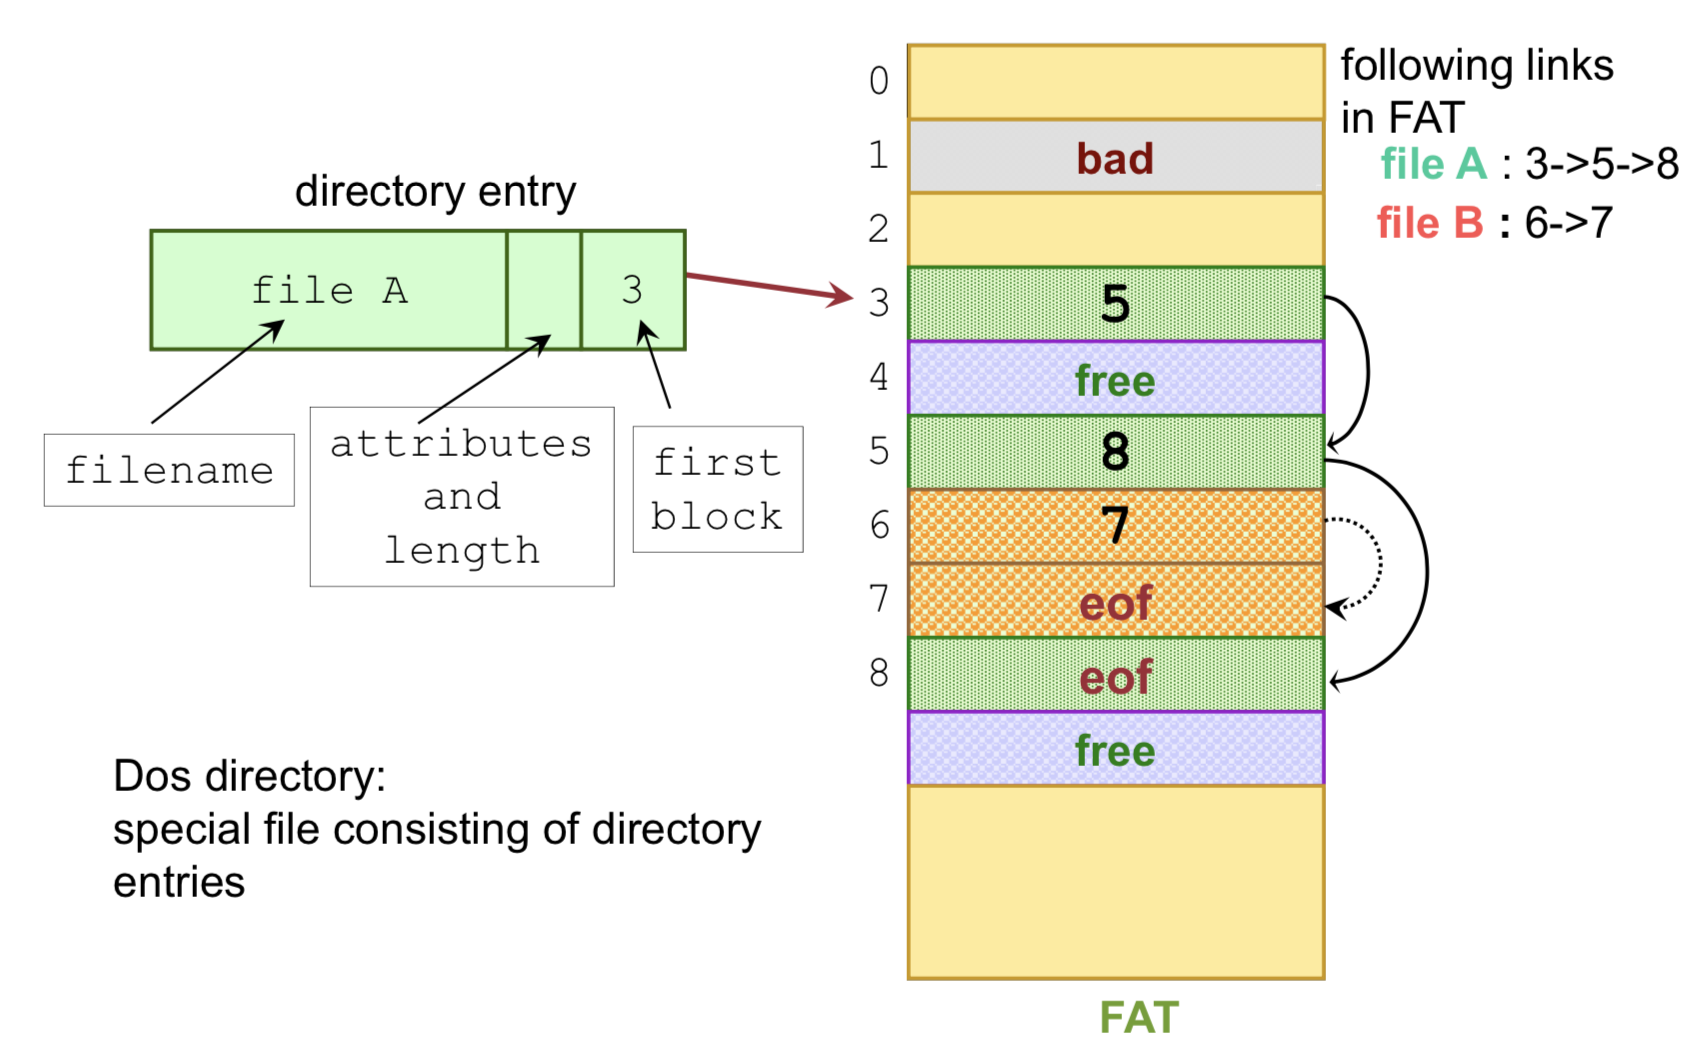
\includegraphics[width=0.9\linewidth]{images/msdos-fat}\\
\emph{Deleting file:} Set first letter in filename to 0xE5, set FAT entries in linked list to FREE.\\
\emph{Cluster:} 16 bits numbers in FAT entries, logical block size=cluster size=multiple of sectors. Large cluster size -> large internal fragmenation.\\
\emph{Disk Fragmenation:} logical contiguous blocks far apart on disk(about time). FAT: less disk fragmentation with large cluster size, solution: run defragmentation(compaction) on entire FS. s5fs: worse since smaller logical block size.

\subsection*{Unix s5fs}
\emph{Inode:} actual file object, one per file. Contains: reference count for hard links, Table of Contents(TOC) mapping file data to disk blocks(hybrid multi-lvl index).\\
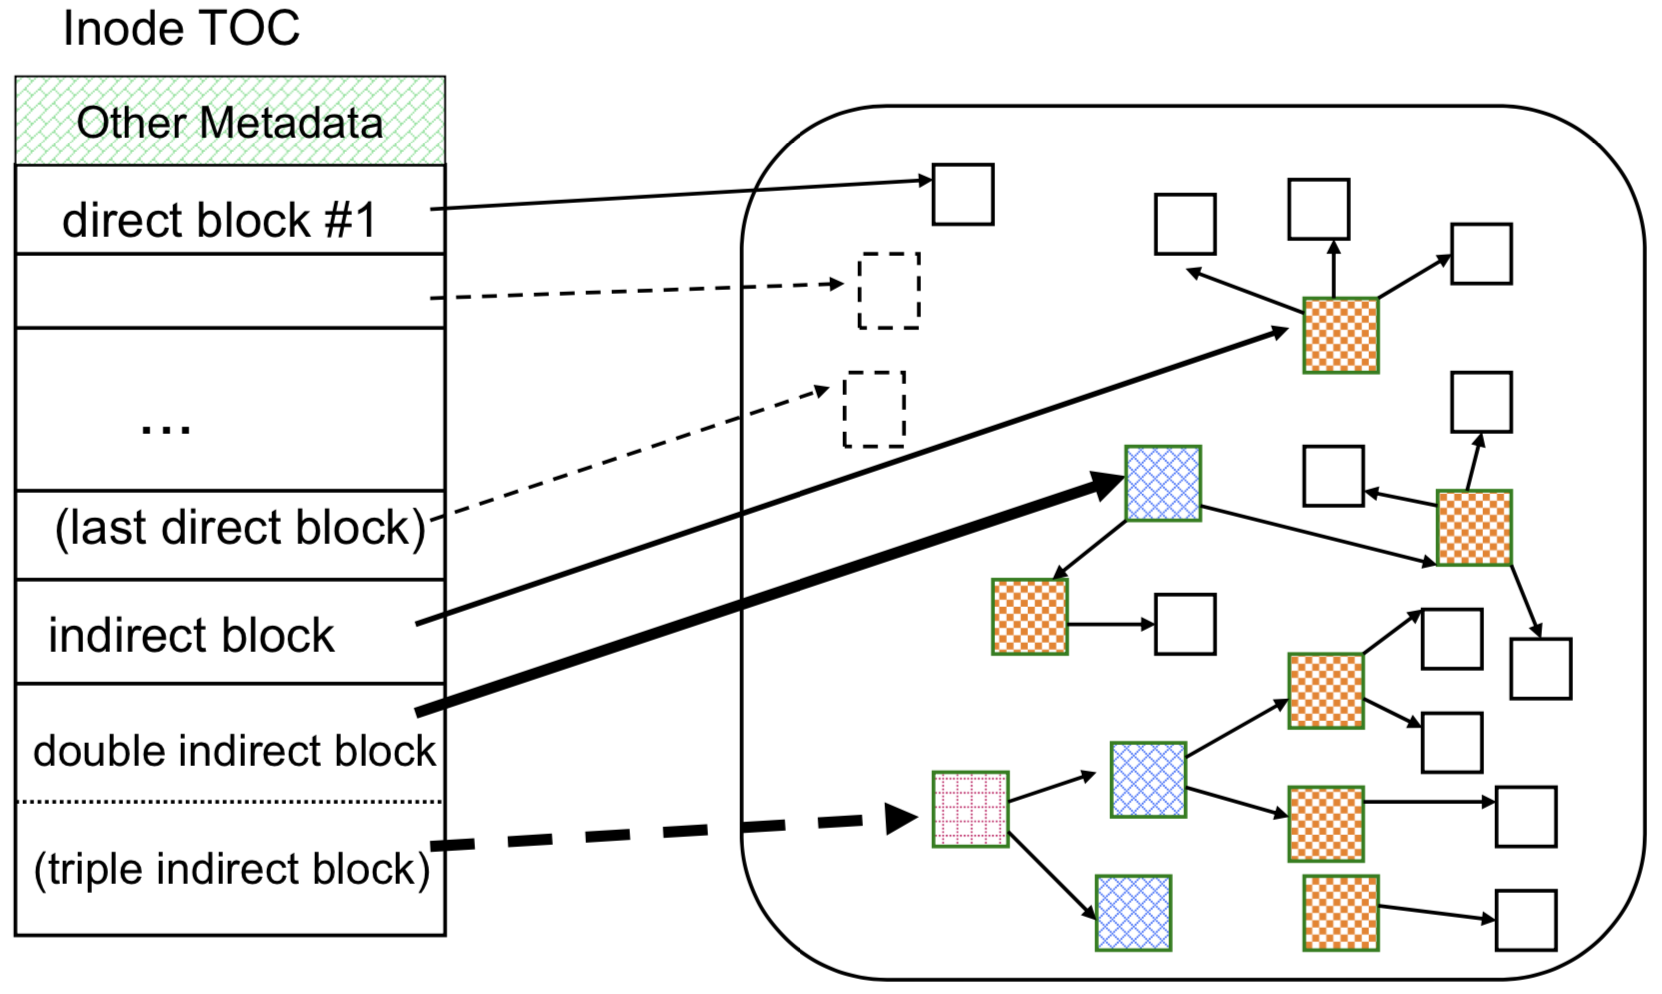
\includegraphics[width=0.9\linewidth]{images/s5fs-toc}\\
Allow blocks which do not exist(logical zero filled holes) - set block pointer to NULL in TOC, return zeroes when read.\\
\emph{Directories:} Map inode \# to filename. Array of 16-byte entries(inode 16 bits, filename 14 bytes). Deleted file has inode 0.\\
\emph{Hard links:} same file to have more than one filename(create DAG). ln. Same inode \# for different filenames. Remove reference with unlink() syscall. Deleting: remove dir entry, decre inode link count, free file object when link count=0.\\
\emph{Caching:} add a buffer cache in memory for disk blocks. Write can be faster than reads(can write to buffer). Use LRU to replace blocks in cache. sync(2) syscall requests dirty buffers be flushed, fsync(2) waits for completion.
\section{Synchronization}
\subsection*{Critical Section (CS)}
\emph{Properties:} Mutual exclusion, progress(if no process in CS, waiting process evetually granted access), bounded wait.\\
\emph{Assumptions:} independence on non-CS, takes finite time.\\
\emph{Problems:} Deadlock, starvation, livelock(keeping changing state with no progress).

\subsection*{Peterson's Algorithm}
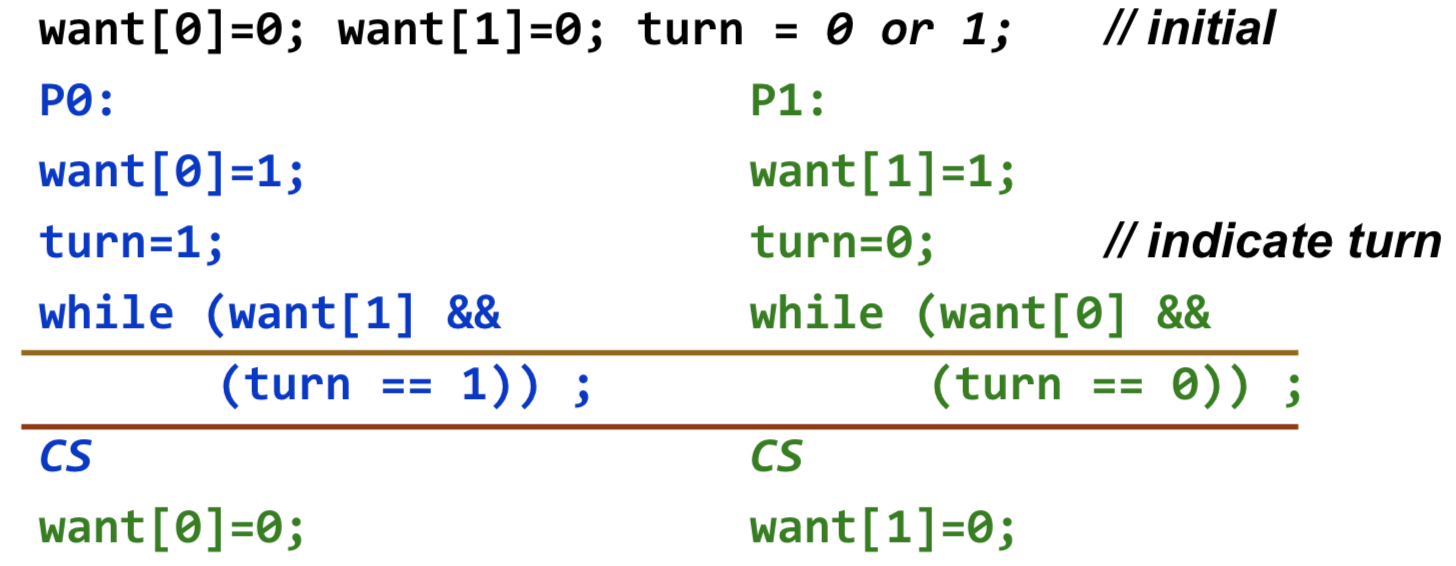
\includegraphics[width=0.6\linewidth]{images/peterson-algo} (-) busy waiting
 
\subsection*{Semaphore}
\emph{Wait() and Signal():}\\
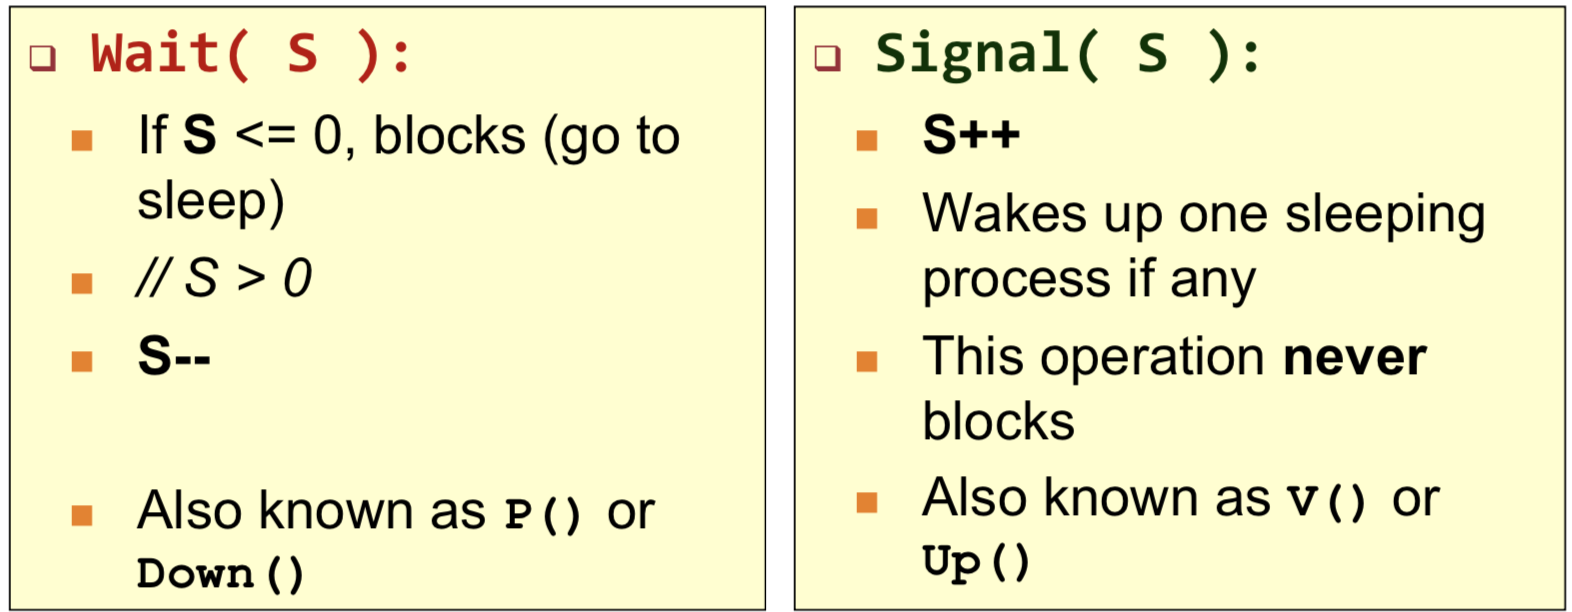
\includegraphics[width=0.75\linewidth]{images/wait-and-signal}\\
$S_{curr}=S_{init}+\#signal(S)-\#wait(S\_comp)$\\
\emph{Mutex:} S=1; Wait(S); CS; Signal(S).

\subsection*{Classic Synchronization Problems}
\emph{Producer Consumer (Blocking):}\\
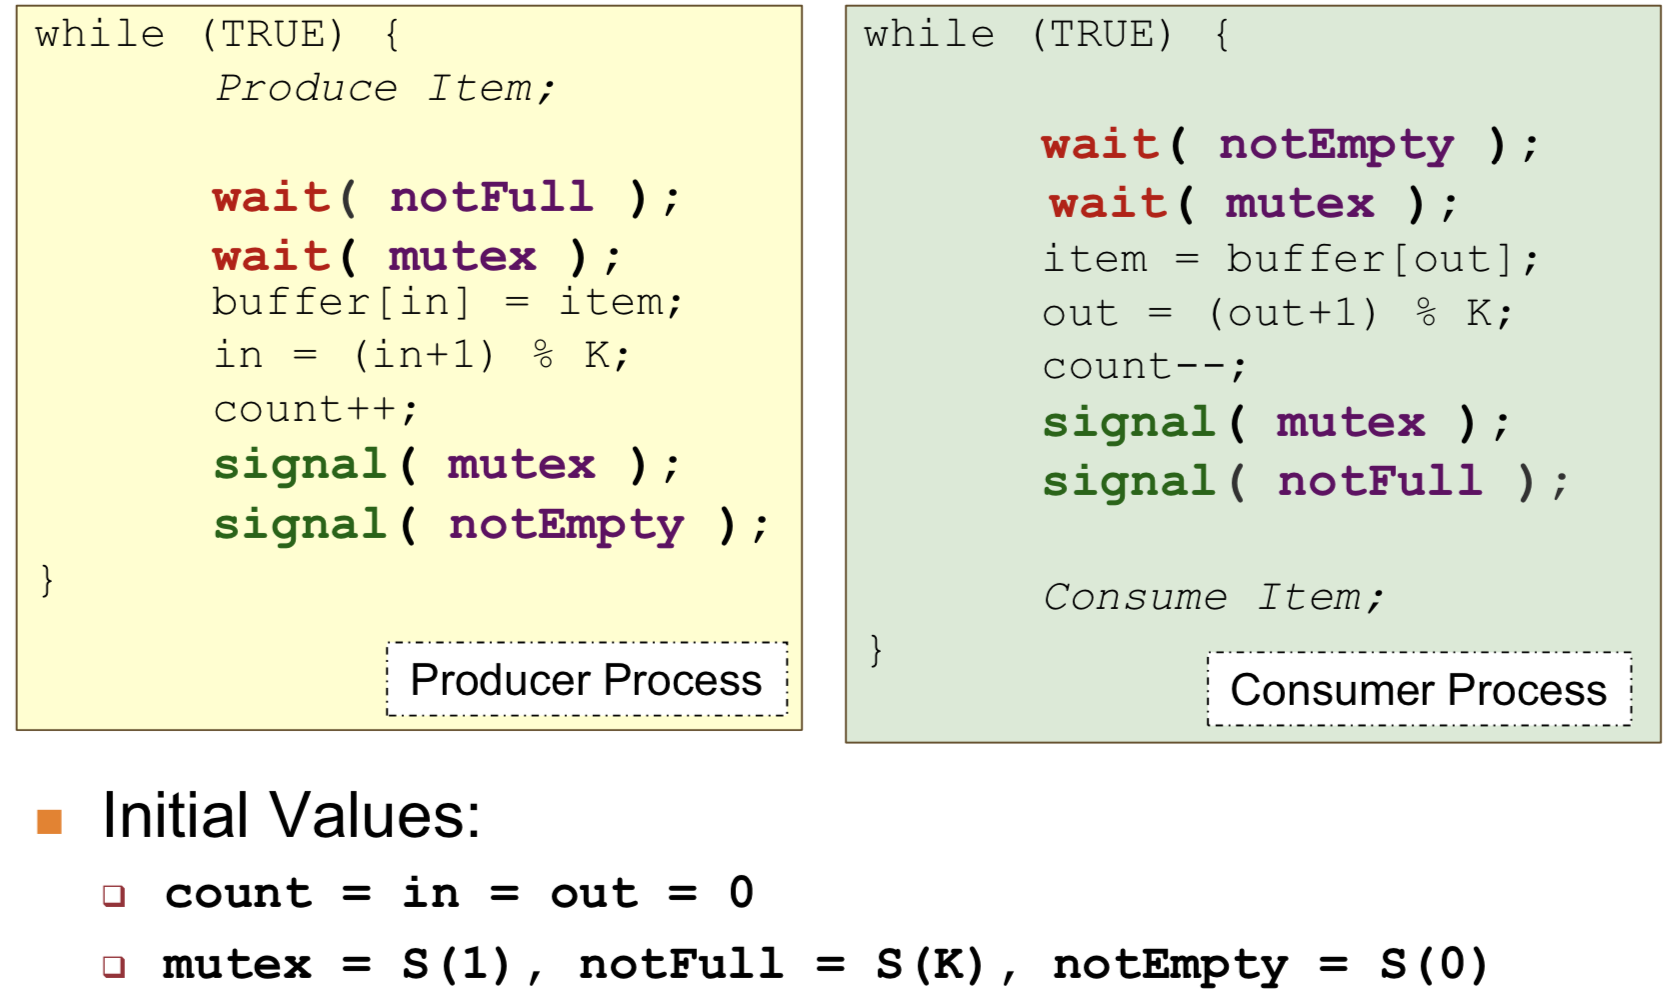
\includegraphics[width=0.75\linewidth]{images/producer-consumer}\\
\emph{Reader Writer:}\\
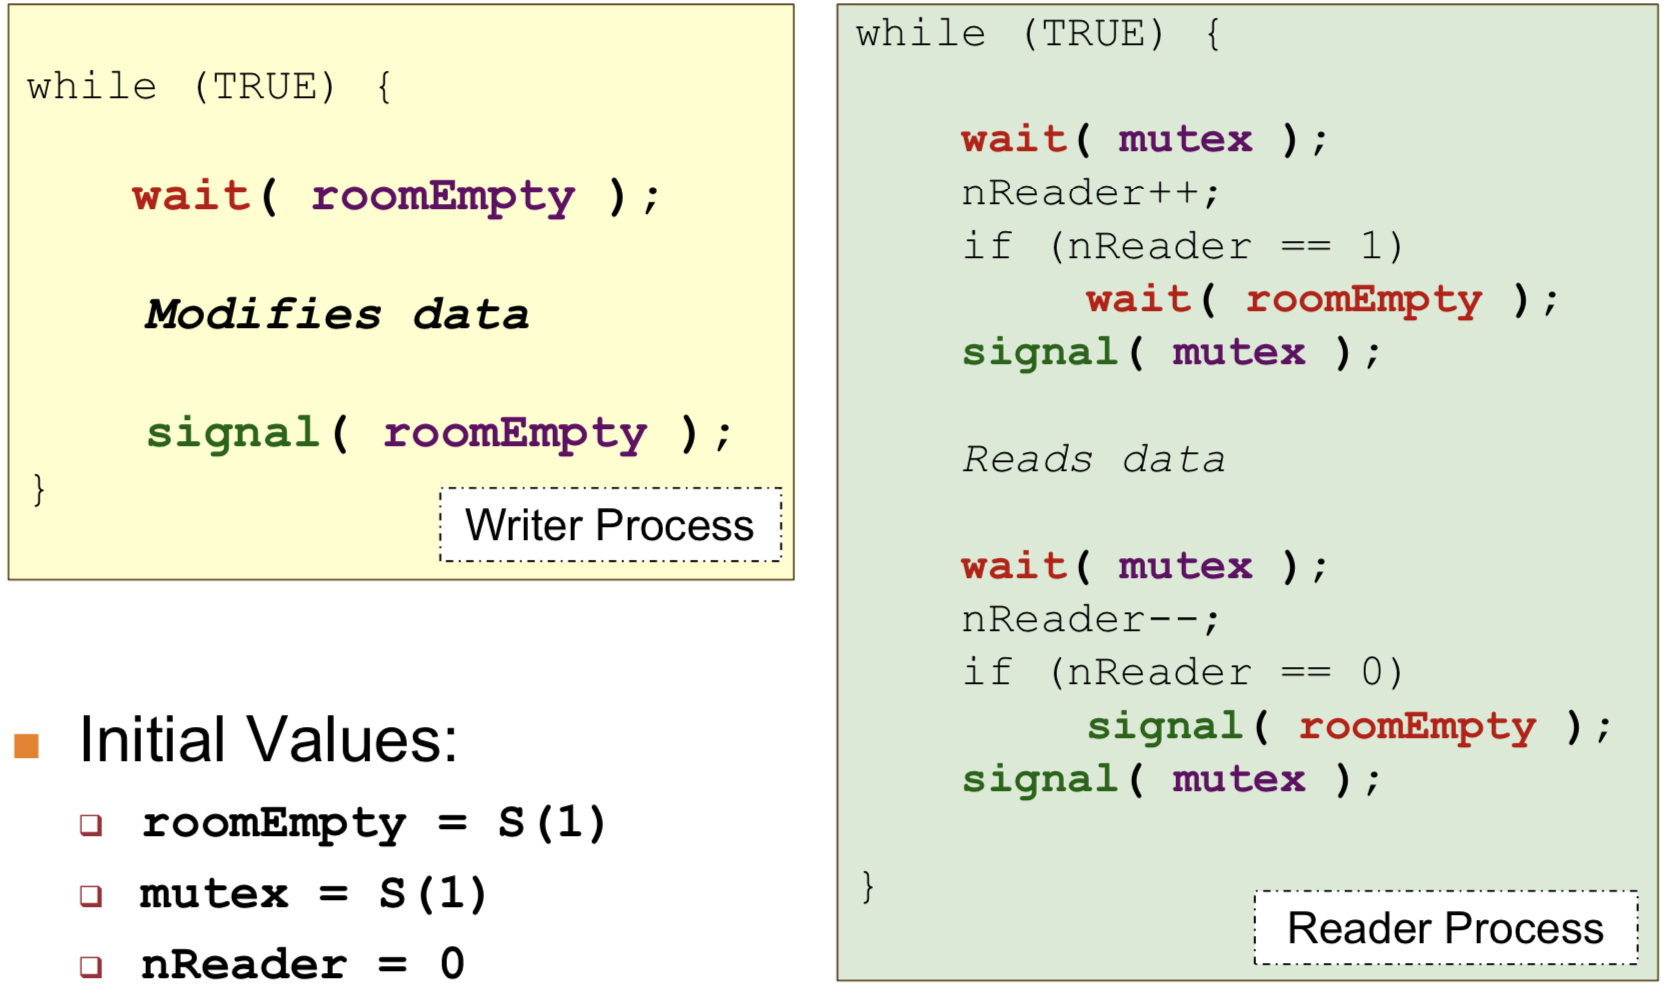
\includegraphics[width=0.75\linewidth]{images/reader-writer}\\
\emph{Dinning Philosopher:}\\
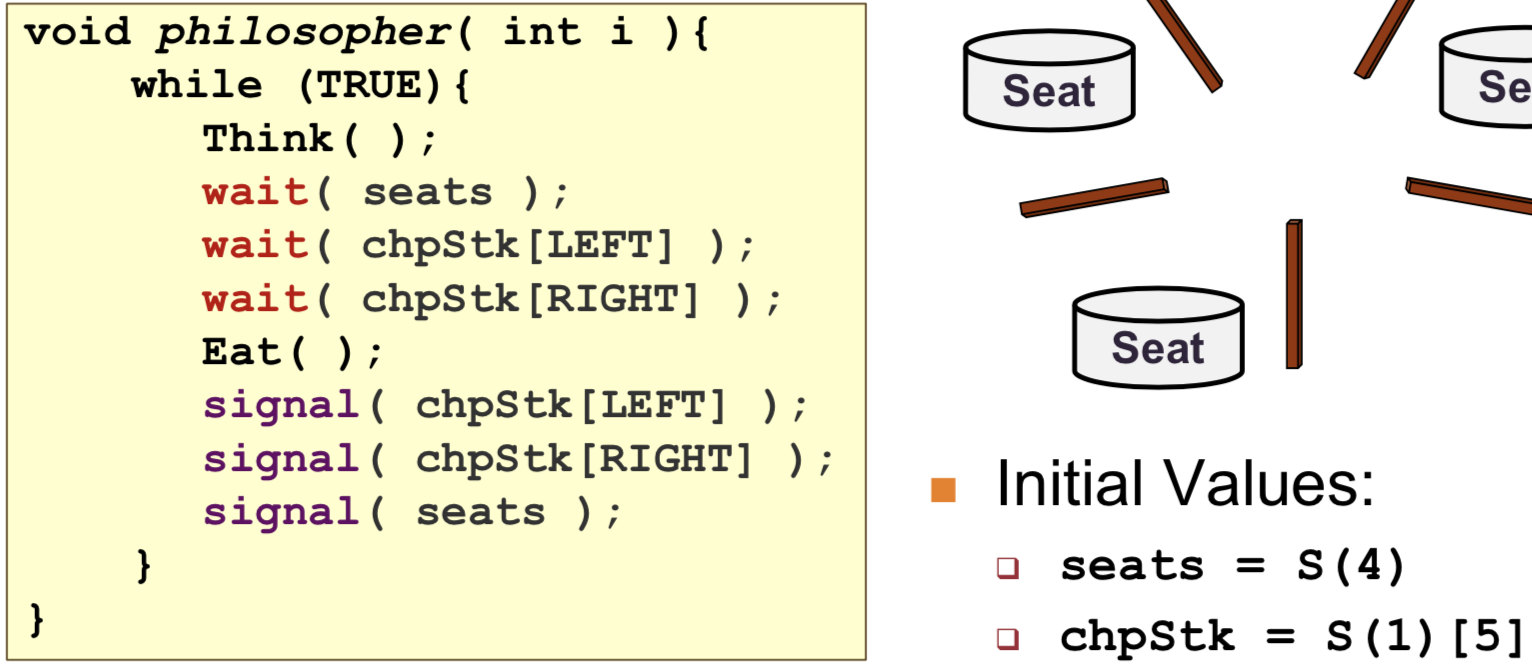
\includegraphics[width=0.75\linewidth]{images/philo-limited-eater}

\subsection *{OS Implementation}
\emph{User mode semaphore implemted by OS:}\\
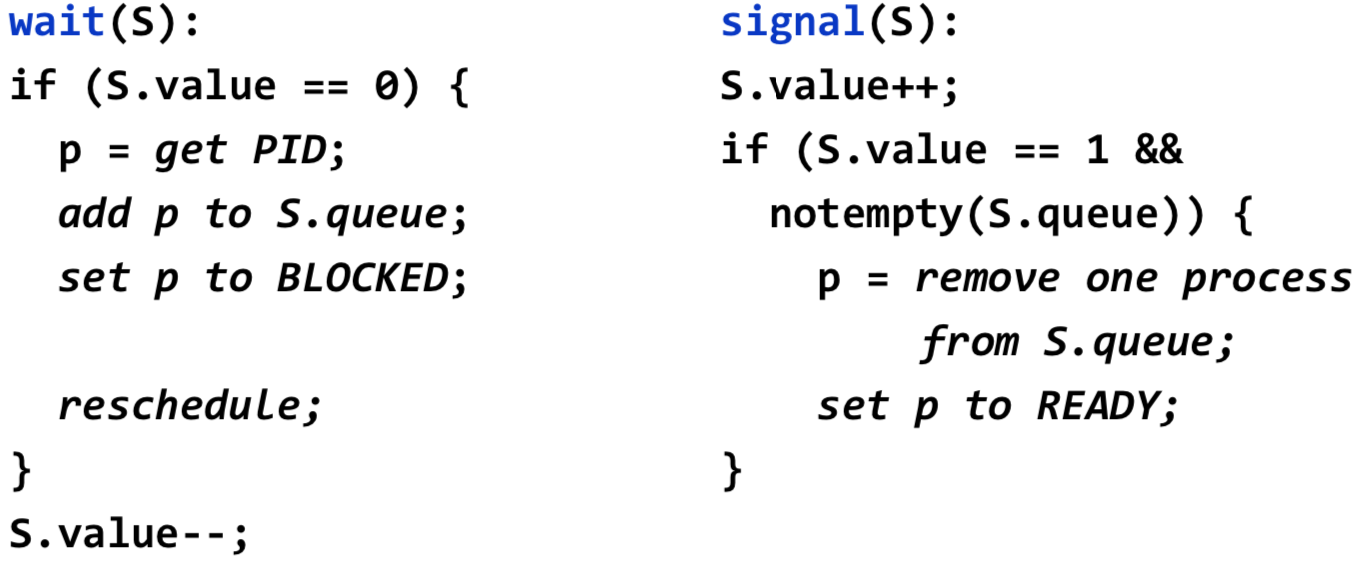
\includegraphics[width=0.75\linewidth]{images/user-semaphore}\\
\emph{Kernel:} disable interrupt(miss interrupt, interfere scheduling)\\
\emph{Multi-processor:} Busy-waiting mutual exclusion(spinlock), HW with atomic read+write\\
\emph{Hardware atomic instruction:} TestAndSet\\
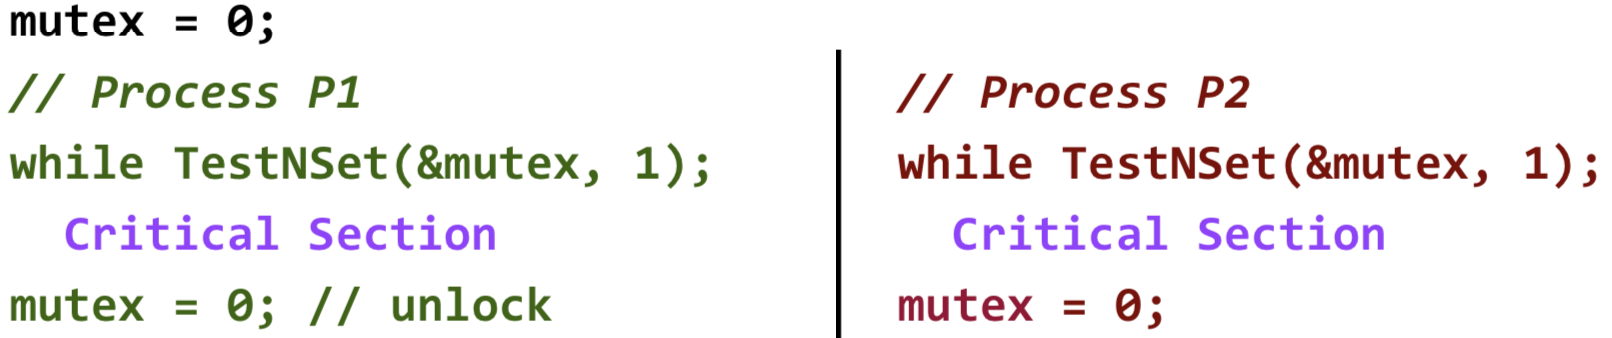
\includegraphics[width=0.7\linewidth]{images/test-and-set} (spinlock)
\end{multicols*}
\end{document}